% ========================
% = Rapport de projet HA =
% ========================
% Joris Berthelot <joris.berthelot@gmail.com>
% Laurent Le Moine <laurent.le.moine17@gmail.com>
% 


\documentclass[11pt,a4paper]{report}
\usepackage{
    content/fullpage, % Enclosed as .sty file
    hyperref,
    listings,
    lmodern,
    fancyhdr,
    algorithmic,
    minted % How to install: http://blog.eexit.net/2011/02/latex-colorez-efficacement-votre-code-source-avec-minted.html
}
%\usepackage[utf8]{inputenc}
\usepackage[T1]{fontenc}
\usepackage[french]{babel}
\usepackage[pdftex]{graphicx}
\pagestyle{fancyplain}
\fancyhf{}
\lhead{\fancyplain{}{Dossier d'Architecture Technique}}
\rhead{\fancyplain{}{Universit\'e de La Rochelle}}
\lfoot{\fancyplain{}{Joris \textsc{BERTHELOT} - Laurent \textsc{LE MOINE}}}
\rfoot{\fancyplain{}{\thepage}}
\definecolor{lightgray}{gray}{.95}
\usemintedstyle{manni}
\newminted{bash}{
    linenos=false,
    bgcolor=lightgray,
    tabsize=4,
    gobble=20,
    fontfamily=courier,
    fontsize=\small,
    xleftmargin=5pt,
    xrightmargin=5pt
}
\hypersetup{
    bookmarks=true,
    unicode=true,
    pdfstartview={FitW}
    pdftitle={Dossier d'Architecture Technique},
    pdfauthor={Joris Berthelot, Laurent Le Moine},
    pdfnewwindow=true,
    colorlinks=true,
    citecolor=black,
    filecolor=black,
    linkcolor=black,
    urlcolor=black
}
\begin{document}
    \newcommand{\HRule}{\rule{\linewidth}{0.5mm}}

\begin{titlepage}

\begin{center}


% Upper part of the page

\includegraphics[width=0.15\textwidth]{content/logo.png}\\[1cm]

\textsc{\LARGE Universit\'e de La Rochelle}\\[1.5cm]

\textsc{\Large Rapport de projet}\\[0.5cm]


% Title
\HRule \\[0.4cm]
{ \huge \bfseries Dossier d'Architecture Technique}\\[0.4cm]

\HRule \\[1.5cm]

% Author and supervisor
\begin{minipage}{0.4\textwidth}
    \begin{flushleft} \large
        \emph{Auteurs:}\\
        Joris \textsc{BERTHELOT}\\
        Laurent \textsc{LE MOINE}
    \end{flushleft}
\end{minipage}
\begin{minipage}{0.4\textwidth}
    \begin{flushright} \large
        \emph{Superviseurs:} \\
        Philippe \textsc{HARRAND}\\
        Bertrand \textsc{VACHON}
    \end{flushright}
\end{minipage}

\vfill

% Bottom of the page
{Master ICONE 2011-2012}

\end{center}

\end{titlepage}
    \newpage
    \setcounter{secnumdepth}{3}
    \setcounter{tocdepth}{4}
    \tableofcontents
    \newpage
    
        \section*{Introduction}
        
        \addcontentsline{toc}{section}{Introduction}
        
        Dans le cadre de notre formation Master Ingéniérie Informatique et de son Unité d'Enseignement Architecture: Conception et Gestion, nous avons réalisé un projet d'architecture réseau HA (High Availability) en 3 jours seulement.\\
        
        Ce projet nous a permis de mettre en exergue nos connaissances récemment acquises lors des cours respectifs de la même UE mais aussi de reprendre et appliquer les concepts vus en TP la semaine auparavant.
        
        \addcontentsline{toc}{section}{Postes de travail}
        
            Assigné comme table n°5, nous avons utilisé les postes suivants :\\
        
            \begin{description}
                \item[Joris Berthelot (sera la machine << JB >> dans le reste du rapport)] \hfill \\
                    \begin{itemize}
                        \item Adresse IP: 10.192.10.23
                        \item Host: mamba13
                    \end{itemize}
                \item[Laurent Le Moine (sera la machine << LLM >> dans le reste du rapport)] \hfill \\
                    \begin{itemize}
                        \item Adresse IP: 10.192.10.24
                        \item Host: mamba14
                    \end{itemize}
            \end{description}
        
        
        \addcontentsline{toc}{section}{Code source}
        
            Etant donné que ce projet fut réalisé en équipe, le code source des différents scripts et fichiers de configuration sont disponible sur Google Code + Subversion. Ainsi, vous pouvez à tout moment récupérer notre travail (ainsi que le code {\LaTeX} du document) comme ceci :\\
            
            \begin{bashcode}
                    svn export http://ulr-acg.googlecode.com/svn/trunk/ ulr-acg-src
            \end{bashcode}
            
    
    \part{Infrastructure logicielle}
        
        Avant toute choses, vous devez savoir que l'ensemble des opérations décrites dans cette section sont a réaliser avec l'utilisateur root. Si vous lancez les scripts livrés avec le rapport sans être root, vous aurez droit à un gentil message d'erreur.\\
        
        Nous avons aussi par ailleurs vidé et désactivé les tables de pare-feu afin de laisse toute nos applications travailler sans avoir de gêne dans un premier temps :\\
        
        \begin{bashcode}
                    # Flushes iptables
                    /sbin/chkconfig --del iptables
                    # Disables firewall service
                    service iptables stop
                    # Enables Network Time Protocol to sync time between machines
                    service ntpd start
        \end{bashcode}
        
        \section{Installation des paquets}
            
            Avant de commencer à configurer et déployer les services, nous aurons besoin d'installer un certain nombre de paquets afin de pouvoir parvenir à nos fins. Aussi divers que variés, nous avons scripté cette installation afin de faciliter la tâche.\\
            
            \subsection{Configuration du proxy}
            
                Il faudra auparavant configurer manuellement les paramètres du proxy si besoin afin de ne pas rendre le script d'installation inopérationnel.
                Pour se faire, veillez à bien changer les paramètres dans les Serveur mandataires (Système > Configuration > Serveurs mandataires) ainsi que rajouter les bons paramètres à Yum (proxy) :\\
                
                \begin{bashcode}
                    # Configuration de Yum
                    vim /etc/yum.conf
                \end{bashcode}
        
        \section{Réplication bas niveau}
            
            La réplication bas niveau permet de créer non pas une redondance applicative mais directement sur le support des données applicatives (système de fichier). L'intêret à cela est d'éviter de configurer chaque service pour sa propre réplication (si existant) et d'aller droit au but en répliquant directement le volume sur lequel repose les données.\\
            
            Voici un petit schéma (issu du site de DRBD) afin d'imager le concept : \\
            
            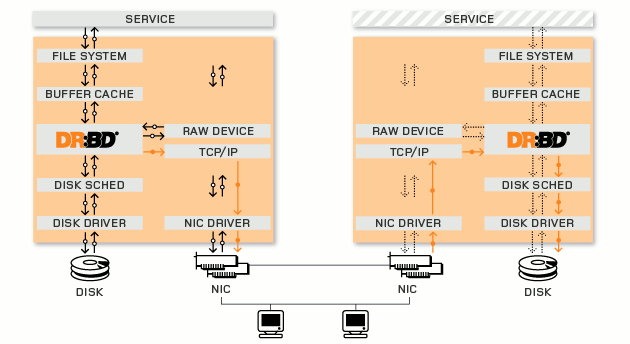
\includegraphics[keepaspectratio=true, width=\textwidth]{content/drbd.png}\\[1cm]
        
            \subsection{Installation}
                
                Pour la réplication bas niveau (système de fichiers), nous avons utilisé \underline{\href{http://www.drbd.org/}{DRBD}} : un logiciel permettant de faire de la réplication de données au sein d'une architecture en grappe. DRBD est assez complexe et fastidieux à mettre en place car il demande quelques notions assez poussées sur les volumes, leur synchronisations, etc.\\
                
                Ce logiciel ne fonctionnait autrefois qu'en mode maître/esclave mais depuis les dernières versions, on peut partir sur une configuration maître/maître afin que les données soient bien synchronisées de manière bidirectionnelle.\\
                
                \begin{bashcode}
                    # Installation de drbd
                    yum install -y drbd drbd-pacemaker drbd-udev
                \end{bashcode}
                
            \subsection{Configuration}
                
                La configuration de DRBD peu s'avérer très simple mais permet un certain degré de complexité en fonction des architectures. La syntaxe est claire et s'apparente à celle du serveur de nom.\\
                Voici la configuration que nous avons utilisé :\\
                
                \inputminted[
                    linenos=true,
                    bgcolor=lightgray,
                    tabsize=4,
                    fontfamily=courier,
                    fontsize=\small,
                    xleftmargin=5pt,
                    xrightmargin=5pt
                ]{bash}{./../confs/drbd/drbd.conf}
                
                DRBD implique qu'un lien réseau doit être établi en supplément des liens existants. Il est important de comprendre que le DRBD utilise un réseau à lui propre afin d'y transférer les données.\\
                
                Pour vérifier que DRBD fonctionne bien, il suffit de voir son état en faisant la commande suivante :\\
                
                \begin{bashcode}
                    cat /proc/drbd
                \end{bashcode}
                
        \section{Déploiement des services}
            
            Dans cette partie, il est important de comprendre que lors de la mise en place d'une architecture en grappe avec des noeuds répliqués, il faut toujours un noeud de référence, surtout dans une architecture active/passive comme celle que nous allons mettre en place.
            Suivant la machine sur laquelle vous allez lancer les scripts, il faudra ou non déployer les données.
        
            \subsection{Apache}
                
                Pour installer Apache, il vous faudra très simplement lancer son script d'installation dans le répertoire \verb+scripts/apache.sh+.
                Ce script va essayer de stopper Apache, vérifier l'intégrité de son fichier de configuration et si il ne concorde pas avec le notre, il va le remplacer. Ensuite, selon si vous êtes le premier noeud de la grappe.
                
            \subsection{MySQL}
            \subsection{DNS}
            \subsection{LDAP}
        \section{Mise en place du pacemaker}
            
            Dans une architecture HA, le système doit pouvoir constamment suivre son état et celui de son entourage afin de décider si il doit basculer (=''failover'') ou non vers un noeud de secours. 
            
    \part{Tests}
        \section{Serveur de noms}
        \section{Serveur Apache}
        \section{Serveur MySQL}
        \section{Serveur LDAP}
    \part{Conclusion}
        \section{Problèmes rencontrés}
        \section{Retours sur échec}
        \section{Retours personnels}
\end{document}